% 第6章第5节：奇异值分解（构造、奇异值与矩阵范数、极分解、最佳低秩逼近）。

\section{奇异值分解}
\label{sec:ls-svd}

前面几节都让输入与输出使用同一组基。在这一要求下用标准正交基换基，只有对称矩阵能化为实对角形，正规矩阵能化为分块对角形，一般方阵只能化为分块上三角的实Schur形。矩形矩阵$\bm A\in\mathbb R^{m\times d}$的输入在$\mathbb R^d$中、输出在$\mathbb R^m$中，“同一组基”与特征向量都无从谈起。于是放宽要求：能否在输入端找一组标准正交方向$\bm v_i$，在输出端找一组标准正交方向$\bm u_i$，使
\[
 \bm A\bm v_i=\sigma_i\bm u_i ,\qquad \sigma_i\geq0,
\]
即$\bm A$只把第$i$个输入方向伸缩$\sigma_i$倍后送到第$i$个输出方向？本节先证明这对任意矩阵都可以做到。所需的方向来自对称矩阵$\bm A^\top\bm A$的特征方向，构造只用到谱定理（定理~\ref{thm:ls-real-symmetric-spectral}）。然后说明这种分解给出了什么：谱范数与Frobenius范数的值，把方阵的作用分成伸缩与转动的极分解，以及给定秩上限时最好的近似。

\subsection{SVD的构造}

先看这样的方向若存在，应当是什么。设$\bm x=\sum_ic_i\bm v_i$，则$\bm A\bm x=\sum_ic_i\sigma_i\bm u_i$，由$\bm u_i$标准正交，
\[
 \bm x^\top\bm A^\top\bm A\bm x=\lVert\bm A\bm x\rVert_2^2=\sum_i\sigma_i^2c_i^2 .
\]
与二次型展开式~\eqref{eq:matrix-analysis-quadratic-spectral-form}比较可知，$\bm v_i$应是对称矩阵$\bm A^\top\bm A$的特征向量，$\sigma_i^2$是对应的特征值。这提示从$\bm A^\top\bm A$出发构造。

令$\bm S=\bm A^\top\bm A$。它对称，而且半正定：$\bm x^\top\bm A^\top\bm A\bm x=\lVert\bm A\bm x\rVert_2^2\geq0$。由谱定理，存在$\mathbb R^d$的标准正交基$\bm v_1,\ldots,\bm v_d$使$\bm A^\top\bm A\bm v_i=\lambda_i\bm v_i$，且$\lambda_1\geq\cdots\geq\lambda_d\geq0$。设前$r$个特征值为正，记$\sigma_i=\sqrt{\lambda_i}>0$（$i\leq r$）。其余的$\bm v_j$满足$\lVert\bm A\bm v_j\rVert_2^2=\bm v_j^\top\bm A^\top\bm A\bm v_j=0$，即$\bm A\bm v_j=\bm0$。

对$i\leq r$定义输出方向$\bm u_i=\bm A\bm v_i/\sigma_i$。它们标准正交：
\[
 \bm u_i^\top\bm u_j
 =\frac{\bm v_i^\top\bm A^\top\bm A\bm v_j}{\sigma_i\sigma_j}
 =\frac{\sigma_j^2\,\bm v_i^\top\bm v_j}{\sigma_i\sigma_j}=\delta_{i,j}.
\]
再把$\bm u_1,\dots,\bm u_r$扩充为$\mathbb R^m$的标准正交基$\bm u_1,\ldots,\bm u_m$。

现在把任意$\bm x$展开为$\bm x=\sum_i(\bm v_i^\top\bm x)\bm v_i$，再利用$\bm A\bm v_i=\sigma_i\bm u_i$（$i\leq r$）与$\bm A\bm v_j=\bm0$（$j>r$），得
\[
 \bm A\bm x=\sum_{i=1}^r\sigma_i\bm u_i(\bm v_i^\top\bm x).
\]
这对所有$\bm x$成立，所以$\bm A$是$r$个秩一矩阵之和：
\begin{equation}
 \bm A=\sum_{i=1}^r\sigma_i\bm u_i\bm v_i^\top.
 \label{eq:matrix-analysis-svd-rank-one-sum}
\end{equation}
由这个和式，$\operatorname{range}(\bm A)$由$\bm u_1,\ldots,\bm u_r$张成；又因为$\bm u_i$线性无关且$\sigma_i>0$，$\bm A\bm x=\bm0$当且仅当$\bm v_i^\top\bm x=0$（$i\leq r$），所以$\ker\bm A$由$\bm v_{r+1},\ldots,\bm v_d$张成。于是$r=\operatorname{rank}\bm A$。把这些向量排成矩阵，就得到下面的结论。

\begin{theorem}[SVD的存在]
\label{thm:ls-svd-existence}
对任意$\bm A\in\mathbb R^{m\times d}$，存在正交矩阵$\bm U\in\mathbb R^{m\times m}$、$\bm V\in\mathbb R^{d\times d}$与对角矩阵$\bm\Sigma\in\mathbb R^{m\times d}$，使$\bm A=\bm U\bm\Sigma\bm V^\top$；$\bm\Sigma$的对角元$\sigma_1\geq\cdots\geq\sigma_{\min(m,d)}\geq0$，其中恰有$\operatorname{rank}\bm A$个为正。
\end{theorem}

\begin{definition}[奇异值分解]
\label{def:matrix-analysis-svd}
称
\begin{equation}
 \bm A=\bm U\bm\Sigma\bm V^\top
 \label{eq:matrix-analysis-svd}
\end{equation}
为$\bm A$的\term{奇异值分解}（singular value decomposition, SVD），$\bm\Sigma$的对角元$\sigma_i$称为\term{奇异值}（singular value），$\bm U$、$\bm V$的列$\bm u_i$、$\bm v_i$分别称为左、右\term{奇异向量}（singular vector）。
\end{definition}

图~\ref{fig:ls-svd-construction}把构造拆成三步：形成$\bm A^\top\bm A$；由谱定理将其对角化；开方得到奇异值，再由$\bm u_i=\bm A\bm v_i/\sigma_i$得到左奇异向量。

\begin{figure*}[htbp]
  \centering
  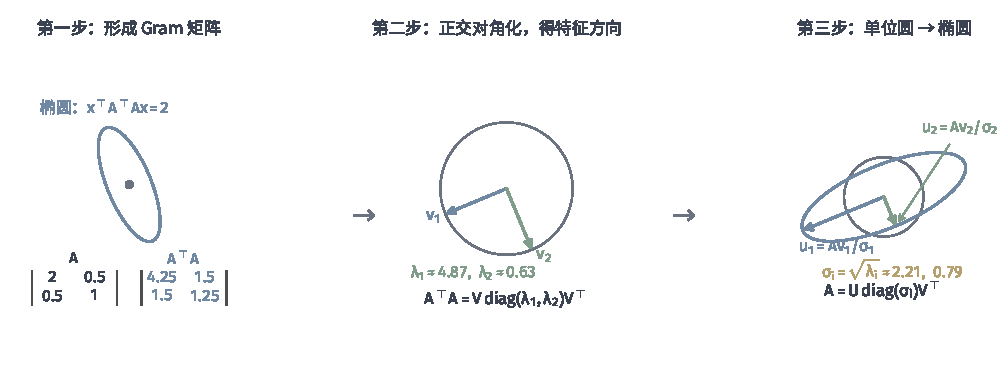
\includegraphics[width=168.998mm]{figures/01-mathematical-preliminaries-upper/03-linear-spaces/matplotlib/ls-svd-construction/ls-svd-construction.pdf}
  \caption{SVD 构造三部曲。以$\bm A=\left[\begin{smallmatrix}2&0.5\\0.5&1\end{smallmatrix}\right]$为例：
  (1)形成$\bm A^\top\bm A=\left[\begin{smallmatrix}4.25&1.5\\1.5&1.25\end{smallmatrix}\right]$；
  (2)由谱定理对角化，特征值$\lambda_1\approx4.87,\lambda_2\approx0.63$；
  (3)$\sigma_i=\sqrt{\lambda_i}\approx2.21,0.79$，右奇异向量$\bm v_i$即特征向量，
  左奇异向量$\bm u_i=\bm A\bm v_i/\sigma_i$。解析式教学构造。}
  \label{fig:ls-svd-construction}
\end{figure*}

几何上，$\bm A$把输入端的单位球面映成输出端的椭球面（秩亏时椭球退化）：$\bm v_i$方向的单位向量被送到长度为$\sigma_i$的半轴$\sigma_i\bm u_i$。图~\ref{fig:matrix-analysis-svd-geometry}用二维旋转矩阵$\bm R(\theta)=\left[\begin{smallmatrix}\cos\theta&-\sin\theta\\\sin\theta&\cos\theta\end{smallmatrix}\right]$构造了一个输入方向与输出方向不同的例子。

\begin{figure*}[htbp]
  \centering
  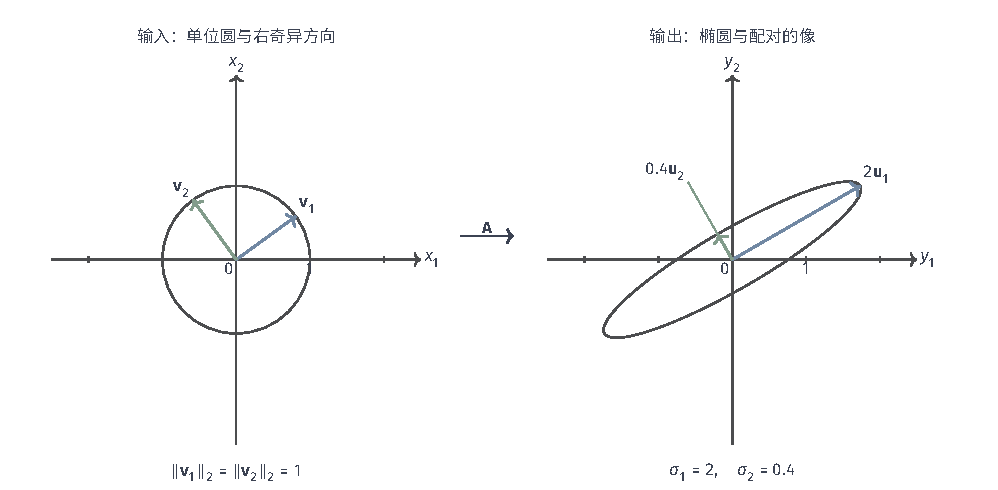
\includegraphics[width=168.998mm]{figures/01-mathematical-preliminaries-upper/03-linear-spaces/tikz/matrix-analysis-svd-geometry/figure.pdf}
  \caption{矩阵$\bm A=\bm R(\pi/6)\operatorname{diag}(2,0.4)\bm R(\pi/5)^\top$
  将单位圆变为椭圆。蓝、绿分别对应两个奇异方向；同色箭头在左侧标出$\bm v_i$，
  在右侧标出其像$\sigma_i\bm u_i$。两侧坐标比例相同。奇异值决定长度变化，左右方向可以不同，
  因而这不是沿特征方向的同空间缩放。图为教学构造。}
  \label{fig:matrix-analysis-svd-geometry}
\end{figure*}

奇异值由$\bm A$唯一确定，它们是$\bm A^\top\bm A$特征值的平方根。奇异向量则不唯一：$\sigma_i$重复时，对应子空间内的任意标准正交基都可以使用；单个$\sigma_i$的一对$\bm u_i,\bm v_i$也可以同时变号。

构造虽然从$\bm A^\top\bm A$出发，数值计算却并不真的形成它：$\bm A^\top\bm A$的特征值是$\sigma_i^2$，小奇异值平方后更小，在舍入中最先失去精度，第~\ref{chap:linear-equations-and-optimization}章讨论最小二乘的数值敏感性时会具体看到这一点。标准算法直接对$\bm A$从两侧施加正交变换，把它化为上双对角形，再迭代求出奇异值；只需要前几个奇异方向时，可以只计算相应的部分。

\subsection{奇异值与矩阵范数}

第~\ref{sec:ls-frobenius-norm}节与第~\ref{sec:ls-matrix-norms}节分别定义了Frobenius范数与谱范数，但没有给出谱范数的算法。SVD直接给出两者的值。对$\bm x=\sum_ic_i\bm v_i$，
\[
 \lVert\bm A\bm x\rVert_2^2=\sum_{i\leq r}\sigma_i^2c_i^2\leq\sigma_1^2\sum_ic_i^2=\sigma_1^2\lVert\bm x\rVert_2^2 ,
\]
等号在$\bm x=\bm v_1$时成立；而$\lVert\bm A\rVert_{\mathrm F}^2=\operatorname{tr}(\bm A^\top\bm A)$等于$\bm A^\top\bm A$的特征值之和$\sum_i\sigma_i^2$。因此
\begin{align}
 \lVert\bm A\rVert_2&=\sigma_1,
 \label{eq:matrix-analysis-spectral-norm}\\
 \lVert\bm A\rVert_{\mathrm F}&=\Bigl(\sum_{i=1}^r\sigma_i^2\Bigr)^{1/2}.
 \label{eq:matrix-analysis-frobenius-norm}
\end{align}
同一展开也给出最弱的放大。$d\leq m$时$\lVert\bm A\bm x\rVert_2\geq\sigma_d\lVert\bm x\rVert_2$，等号在$\bm x=\bm v_d$时成立，秩亏时$\sigma_d=0$。对可逆方阵，$\bm A^{-1}=\sum_i\sigma_i^{-1}\bm v_i\bm u_i^\top$（直接相乘可验证$\bm A\bm A^{-1}=\sum_i\bm u_i\bm u_i^\top=\bm I$），它的最大奇异值是$1/\sigma_d$，所以$\lVert\bm A^{-1}\rVert_2=1/\sigma_d$。

最大奇异值衡量最强的放大，最小奇异值衡量最弱的放大，二者之比就是第~\ref{sec:ls-perturbation-conditioning}节的条件数。齐次最小二乘~\eqref{eq:linear-algebra-homogeneous-least-squares}的最优解也可以由此读出：它是$\bm V$的最后一列$\bm v_d$，因为按构造，$\bm v_d$是$\bm A^\top\bm A$最小特征值的单位特征向量。

\subsection{极分解}

SVD还可以把方阵的作用分成“伸缩”与“转动”两步，类似于把复数写成模长与单位复数之积。设$\bm A\in\mathbb R^{d\times d}$有SVD$\bm A=\bm U\bm\Sigma\bm V^\top$，在$\bm U$与$\bm\Sigma$之间插入$\bm V^\top\bm V=\bm I$，得$\bm A=(\bm U\bm V^\top)(\bm V\bm\Sigma\bm V^\top)$。
\begin{definition}[极分解]
\label{def:matrix-analysis-polar-decomposition}
方阵$\bm A$的\term{极分解}（polar decomposition）是
\begin{equation}
 \bm A=\bm W\bm H,\qquad \bm W=\bm U\bm V^\top,\quad \bm H=\bm V\bm\Sigma\bm V^\top=(\bm A^\top\bm A)^{1/2},
 \label{eq:matrix-analysis-polar-decomposition}
\end{equation}
其中$\bm W$正交，$\bm H$对称半正定。
\end{definition}
$\bm H$先沿$\bm v_i$方向伸缩，$\bm W$再作正交变换。由$\bm H^2=\bm V\bm\Sigma^2\bm V^\top=\bm A^\top\bm A$及半正定平方根的唯一性，$\bm H$由$\bm A$唯一确定；$\bm A$可逆时$\bm H$可逆，$\bm W=\bm A\bm H^{-1}$也唯一。

正交因子$\bm W$是Frobenius范数下离$\bm A$最近的正交矩阵。对正交$\bm Z$，$\lVert\bm Z\rVert_{\mathrm F}^2=d$，展开得$\lVert\bm A-\bm Z\rVert_{\mathrm F}^2=\lVert\bm A\rVert_{\mathrm F}^2+d-2\operatorname{tr}(\bm Z^\top\bm A)$，所以只需让$\operatorname{tr}(\bm Z^\top\bm A)$最大。由迹的循环性，
\[
 \operatorname{tr}(\bm Z^\top\bm U\bm\Sigma\bm V^\top)=\operatorname{tr}(\bm V^\top\bm Z^\top\bm U\,\bm\Sigma)=\sum_i\sigma_i(\bm V^\top\bm Z^\top\bm U)_{i,i}.
\]
$\bm V^\top\bm Z^\top\bm U$是正交矩阵，其列是单位向量，对角元不超过$1$，故迹不超过$\sum_i\sigma_i$；取$\bm Z=\bm U\bm V^\top$时该矩阵为$\bm I$，等号成立。含噪的旋转估计常用这一步把近似正交的矩阵修正为正交矩阵。

\subsection{最佳低秩逼近}
\label{sec:ls-low-rank-solve}
\label{sec:ls-full-svd-solve}
\label{sec:matrix-analysis-svd-low-rank}

数据矩阵常常近似低秩：少数几个方向承载了大部分信息。给定秩上限$k$，怎样找离$\bm A$最近的秩不超过$k$的矩阵？秩一分解~\eqref{eq:matrix-analysis-svd-rank-one-sum}把$\bm A$按奇异值从大到小拆成$r$项，一个自然的候选是只保留前$k$项。

设$\bm A\in\mathbb R^{m\times d}$的非零奇异值为$\sigma_1\geq\cdots\geq\sigma_r>0$，称
\begin{equation}
 \bm A_k=\sum_{i=1}^k\sigma_i\bm u_i\bm v_i^\top,
 \qquad 0\leq k<r
 \label{eq:matrix-analysis-truncated-svd}
\end{equation}
为\term{截断SVD}（truncated SVD），$k=0$时$\bm A_0=\bm0$。

余下的$\bm A-\bm A_k=\sum_{i>k}\sigma_i\bm u_i\bm v_i^\top$本身就是一个SVD，最大奇异值为$\sigma_{k+1}$，由式~\eqref{eq:matrix-analysis-spectral-norm}与式~\eqref{eq:matrix-analysis-frobenius-norm}直接读出两种误差：
\begin{equation}
 \lVert\bm A-\bm A_k\rVert_2=\sigma_{k+1},\qquad
 \lVert\bm A-\bm A_k\rVert_{\mathrm F}
 =\Bigl(\sum_{i=k+1}^r\sigma_i^2\Bigr)^{1/2}.
 \label{eq:ls-truncated-errors}
\end{equation}
谱范数误差是最坏单位输入的输出偏差，Frobenius误差累计全部元素的平方偏差。下面的定理说明，在这两种范数下没有比截断SVD更好的秩$k$近似。

\begin{theorem}[Eckart--Young--Mirsky最佳低秩逼近]
\label{thm:ls-best-low-rank}
\label{thm:matrix-analysis-best-low-rank}
对$0\leq k<r=\operatorname{rank}\bm A$，
\begin{align}
 \min_{\operatorname{rank}\bm B\leq k}\lVert\bm A-\bm B\rVert_2
 &=\sigma_{k+1},
 \label{eq:matrix-analysis-best-rank-k-spectral}\\
 \min_{\operatorname{rank}\bm B\leq k}\lVert\bm A-\bm B\rVert_{\mathrm F}
 &=\Bigl(\sum_{i=k+1}^r\sigma_i^2\Bigr)^{1/2},
 \label{eq:matrix-analysis-best-rank-k-frobenius}
\end{align}
两个最小值都由截断SVD$\bm A_k$达到。
\end{theorem}
\begin{proof}
式~\eqref{eq:ls-truncated-errors}说明$\bm A_k$达到右端，只需证明任意秩不超过$k$的$\bm B$误差都不更小。$k=0$时$\bm B=\bm0$，结论即式~\eqref{eq:ls-truncated-errors}，下设$k\geq1$。

谱范数情形。$\ker\bm B$的维数至少为$d-k$，子空间$\operatorname{span}\{\bm v_1,\ldots,\bm v_{k+1}\}$的维数为$k+1$，两者维数之和超过$d$，必有公共单位向量$\bm x=\sum_{i=1}^{k+1}c_i\bm v_i$，$\sum_ic_i^2=1$。由$\bm B\bm x=\bm0$，
\begin{equation}
 \lVert(\bm A-\bm B)\bm x\rVert_2
 =\lVert\bm A\bm x\rVert_2
 =\Bigl(\sum_{i=1}^{k+1}\sigma_i^2c_i^2\Bigr)^{1/2}
 \geq\sigma_{k+1},
 \label{eq:ls-spectral-lower-bound}
\end{equation}
所以$\lVert\bm A-\bm B\rVert_2\geq\sigma_{k+1}$。

Frobenius情形。正交变换不改变Frobenius范数，令$\bm C=\bm U^\top\bm B\bm V$，则$\operatorname{rank}\bm C=\operatorname{rank}\bm B\leq k$，且$\lVert\bm A-\bm B\rVert_{\mathrm F}=\lVert\bm\Sigma-\bm C\rVert_{\mathrm F}$。设$\bm P$为到$\bm C$列空间的正交投影，则$\operatorname{tr}\bm P=\operatorname{rank}\bm C\leq k$，且$\bm P\bm C=\bm C$。把$\bm\Sigma-\bm C$拆成$(\bm I-\bm P)\bm\Sigma$与$\bm P\bm\Sigma-\bm C$，两部分的每一列分别落在互相正交的子空间中，于是
\[
 \lVert\bm\Sigma-\bm C\rVert_{\mathrm F}^2
 =\lVert(\bm I-\bm P)\bm\Sigma\rVert_{\mathrm F}^2+\lVert\bm P\bm\Sigma-\bm C\rVert_{\mathrm F}^2
 \geq\lVert\bm\Sigma\rVert_{\mathrm F}^2-\lVert\bm P\bm\Sigma\rVert_{\mathrm F}^2 .
\]
$\bm\Sigma$的第$i$列是$\sigma_i\bm e_i$，所以保留部分为$\lVert\bm P\bm\Sigma\rVert_{\mathrm F}^2=\sum_i\sigma_i^2w_i$，其中$w_i=\lVert\bm P\bm e_i\rVert_2^2\in[0,1]$，且$\sum_iw_i\leq\lVert\bm P\rVert_{\mathrm F}^2=\operatorname{tr}\bm P\leq k$。与迹极值定理的证明相同，由$\sigma_i$降序，
\[
 \sum_i\sigma_i^2w_i-\sum_{i\leq k}\sigma_i^2
 =\sum_{i\leq k}\sigma_i^2(w_i-1)+\sum_{i>k}\sigma_i^2w_i
 \leq\sigma_k^2\Bigl(\sum_iw_i-k\Bigr)\leq0 .
\]
即保留部分不超过$\sum_{i\leq k}\sigma_i^2$，误差平方至少为$\lVert\bm\Sigma\rVert_{\mathrm F}^2-\sum_{i\leq k}\sigma_i^2=\sum_{i>k}\sigma_i^2$。
\end{proof}
这一结论最早由Eckart与Young给出\scite{eckart1936}。上面的证明只处理谱范数与Frobenius范数；误差改用加权、逐元素或分组的度量时，最优性需要重新论证，截断SVD一般不再是最优解。图~\ref{fig:ls-low-rank-truncation}画出截断的几何：单位圆经$\bm A$变成椭圆，秩一近似把椭圆压成主轴方向的线段，残留误差恰为舍弃的$\sigma_2$。

\begin{figure*}[htbp]
  \centering
  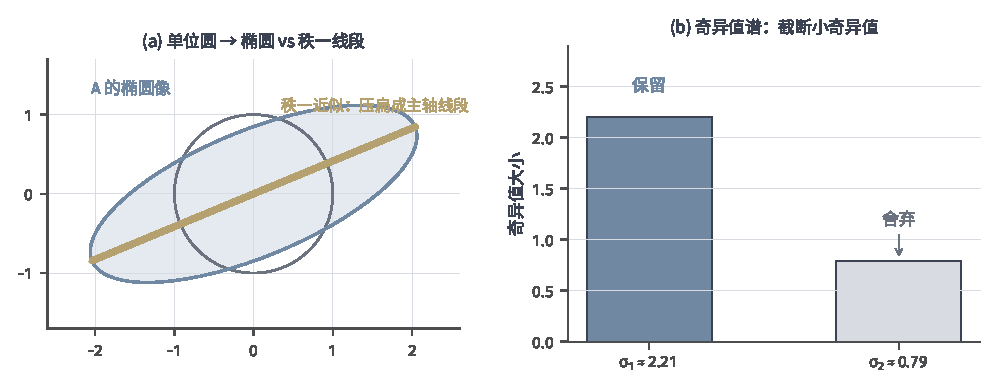
\includegraphics[width=168.998mm]{figures/01-mathematical-preliminaries-upper/03-linear-spaces/matplotlib/ls-low-rank-truncation/ls-low-rank-truncation.pdf}
  \caption{低秩截断的几何。$\bm A=\left[\begin{smallmatrix}2&0.5\\0.5&1\end{smallmatrix}\right]$，
  灰圆为单位圆，蓝椭圆为$\bm A$的像。左：黄粗线段为秩一近似$\bm A_1=\sigma_1\bm v_1\bm v_1^\top$
  的像，椭圆被压成长$2\sigma_1$的线段；右：$\sigma_1\approx2.21$（保留）、$\sigma_2\approx0.79$
  （舍弃），算子范数误差$\lVert\bm A-\bm A_1\rVert_2=\sigma_2$。$\sigma_{1,2}=(3\pm\sqrt2)/2$。
  固定复算。}
  \label{fig:ls-low-rank-truncation}
\end{figure*}

回到本节开头的问题：任意矩阵都能写成$\bm A=\sum_{i\leq r}\sigma_i\bm u_i\bm v_i^\top$，在输入、输出两侧各取一组标准正交方向后，它只是逐个方向的伸缩。奇异值由$\bm A$唯一确定，最大奇异值是谱范数，平方和是Frobenius范数的平方，最小奇异值衡量最弱的放大；方阵还可以写成正交因子与半正定因子之积；按奇异值从大到小截断，得到谱范数与Frobenius范数下的最佳低秩逼近。同一个和式还能反过来用：把每一项$\sigma_i\bm u_i\bm v_i^\top$换成$\sigma_i^{-1}\bm v_i\bm u_i^\top$，就得到秩亏、不相容方程的最小范数最小二乘解，这一构造留到第~\ref{chap:linear-equations-and-optimization}章与线性方程的求解一起讨论。

到这里，本章的第一个问题告一段落：由特征向量组成的基（若存在）使算子的矩阵成为对角形；要求基标准正交时，对称矩阵仍能对角化，一般方阵只能化为实Schur形；输入、输出各取一组标准正交基时，任意矩阵都能对角化。后面三节用这些最简形式研究线性作用的性质，首先是一次作用对误差的放大。最强与最弱的放大分别由最大与最小奇异值给出，下一节用它们定义条件数。
